\documentclass{article}

% Pacotes
\usepackage[utf8]{inputenc}
\usepackage[brazil]{babel}
\usepackage[letterpaper,top=2.5cm,bottom=2.5cm,left=3cm,right=3cm,marginparwidth=1.75cm]{geometry}
\usepackage{amsmath, graphicx, subcaption}
\usepackage[colorlinks=true, allcolors=blue]{hyperref}

\usepackage{listings}
\usepackage{xcolor}
\usepackage{tabularx}
\usepackage{array}
\usepackage{amssymb}    % símbolos matemáticos extras
\usepackage{url}
\usepackage{booktabs}   % Para top/mid/bottomrule
\usepackage{float}      % Para [H]
\usepackage{enumitem}   % Para customizar listas (a), (b), (c)


% Definições de estilo para Python
\lstdefinestyle{pythonstyle}{
      language=Python,
      basicstyle=\ttfamily\small,
      keywordstyle=\color{blue}\bfseries,
      commentstyle=\color{gray}\itshape,
      stringstyle=\color{orange},
      numbers=left,
      numberstyle=\tiny,
      stepnumber=1,
      numbersep=10pt,
      backgroundcolor=\color{white},
      frame=single,
      breaklines=true,
      tabsize=4,
      showstringspaces=false,
      % Permite acentos e símbolos nos comentários do código
      literate={á}{{\'a}}1 {à}{{\`a}}1 {ã}{{\~a}}1 {â}{{\^a}}1
               {é}{{\'e}}1 {ê}{{\^e}}1 {í}{{\'i}}1 {ó}{{\'o}}1
               {õ}{{\~o}}1 {ô}{{\^o}}1 {ú}{{\'u}}1 {ç}{{\c{c}}}1
               {Á}{{\'A}}1 {É}{{\'E}}1 {Í}{{\'I}}1 {Ó}{{\'O}}1
               {Ú}{{\'U}}1 {Ç}{{\c{C}}}1 {º}{{$^{\circ}$}}1,
}

\renewcommand{\lstlistingname}{Listagem}
\setlength{\emergencystretch}{2em} % evita linhas estouradas com trechos de código no texto

\begin{document}

% Capa personalizada
\begin{titlepage}
      \centering
      \IfFileExists{images/fig_logo_cefetmg.pdf}{\includegraphics[width=4cm]{images/fig_logo_cefetmg.pdf}\par}{}
      \vspace{0.5cm}

      {\LARGE Centro Federal de Educação Tecnológica de Minas Gerais \par}
      \vspace{0.2cm}

      {\Large Engenharia de Computação \\ Computação Gráfica \par}
      \vspace{4cm}

      {\Huge \textbf{Relatório de Desenvolvimento} \par}
      \vspace{0.5cm}

      {\LARGE Visualização 3D de uma Pirâmide e de um Prisma com GLFW e OpenGL \par}
      \vspace{3cm}

      {\LARGE João Paulo da Cunha Faria \par}
      {\LARGE Maria Eduarda Teixeira Souza \par}
      \vfill

      {\large Divinópolis - MG \par}
      {\large Outubro de 2026 \par}
\end{titlepage}


\section{Introdução}

Na Aula 15 foi apresentada a biblioteca GLFW (\textit{Graphics Library Framework}), que faz a ponte entre o OpenGL e o Sistema Operacional. Como exemplo, o professor mostrou o programa \texttt{cubo\_3d.py}, que desenha um cubo azul em 3D dentro de uma janela e permite girá-lo com as setas do teclado. Ao final da aula, foi proposta a seguinte atividade: \textit{``implemente a visualização 3D de uma pirâmide e de um prisma''}.

Para resolver a atividade, foram criados dois programas em \textit{Python}, \texttt{piramide\_3d.py} e \texttt{prisma\_3d.py}, que seguem a mesma estrutura do cubo visto em aula. O que muda de um programa para o outro é apenas a geometria do sólido: a lista de vértices, as cores de cada face e a forma como os vértices são ligados em triângulos. Este relatório explica como os dois programas foram construídos e mostra o resultado da execução de cada um.

\section{Fundamentação}

\subsection{O Papel do GLFW}

O OpenGL sabe apenas fazer cálculos na placa de vídeo para pintar pixels: ele não sabe o que é uma janela, um teclado ou um mouse. Por isso, sozinho, ele não consegue nem abrir uma tela preta no monitor. Como visto em aula, o GLFW assume três responsabilidades que completam o OpenGL:

\begin{enumerate}
    \item \textbf{Criação da janela:} cada sistema operacional cria janelas de um jeito diferente (Win32 no Windows, X11 ou Wayland no Linux, Cocoa no macOS). A função \texttt{glfw.create\_window()} esconde essas diferenças;
    \item \textbf{Criação do contexto OpenGL:} o GLFW negocia com o driver da placa de vídeo a versão do OpenGL que será usada (neste trabalho, a versão 3.3 no perfil \textit{Core});
    \item \textbf{Leitura do teclado e do mouse:} é o GLFW que percebe quando uma tecla foi pressionada e repassa essa informação para o programa, através de \texttt{glfw.poll\_events()} e \texttt{glfw.get\_key()}.
\end{enumerate}

\subsection{Coordenadas Homogêneas em 3D}

Na Aula 14 foi visto que a translação não pode ser feita só com multiplicação de matrizes, pois ela é uma soma. A solução é acrescentar uma coordenada extra $w$ ao ponto. Em 3D, um ponto $(x, y, z)$ passa a ser escrito como $[x,\ y,\ z,\ 1]^T$ e todas as transformações viram matrizes $4\times4$. As matrizes usadas neste trabalho são a translação $T$ e as rotações em torno dos eixos $X$ e $Y$:

\begin{equation}\label{eq:matrizes}
T = \begin{bmatrix} 1 & 0 & 0 & t_x \\ 0 & 1 & 0 & t_y \\ 0 & 0 & 1 & t_z \\ 0 & 0 & 0 & 1 \end{bmatrix}, \quad
R_x = \begin{bmatrix} 1 & 0 & 0 & 0 \\ 0 & \cos\theta & -\sin\theta & 0 \\ 0 & \sin\theta & \cos\theta & 0 \\ 0 & 0 & 0 & 1 \end{bmatrix}, \quad
R_y = \begin{bmatrix} \cos\theta & 0 & \sin\theta & 0 \\ 0 & 1 & 0 & 0 \\ -\sin\theta & 0 & \cos\theta & 0 \\ 0 & 0 & 0 & 1 \end{bmatrix}
\end{equation}

Também foi visto que um ponto homogêneo $(x', y', z', w)$ volta para o sistema cartesiano dividindo as três primeiras coordenadas por $w$:

\begin{equation}\label{eq:divisao}
(x, y, z) = \left(\frac{x'}{w},\ \frac{y'}{w},\ \frac{z'}{w}\right), \qquad w \neq 0
\end{equation}

Enquanto $w = 1$, essa divisão não muda nada. Ela passa a ser importante na projeção em perspectiva, explicada a seguir.

\subsection{A Matriz MVP}

Para desenhar um sólido 3D na tela, cada vértice passa por três matrizes, que juntas formam a matriz MVP (\textit{Model}, \textit{View}, \textit{Projection}):

\begin{equation}\label{eq:mvp}
MVP = P \cdot V \cdot M \qquad \Rightarrow \qquad P_{tela} = MVP \cdot [x,\ y,\ z,\ 1]^T
\end{equation}

\begin{itemize}
    \item \textbf{Model ($M$):} gira o sólido. Neste trabalho, $M = R_x(\theta_x) \cdot R_y(\theta_y)$, onde os ângulos mudam conforme as setas do teclado;
    \item \textbf{View ($V$):} representa a câmera. Como no OpenGL a câmera olha para $-z$, o sólido é afastado com $V = T(0, 0, -3{,}5)$, o que equivale a recuar a câmera 3,5 unidades;
    \item \textbf{Projection ($P$):} aplica a perspectiva, fazendo com que as partes mais distantes apareçam menores:
\end{itemize}

\begin{equation}\label{eq:perspectiva}
P = \begin{bmatrix}
\dfrac{f}{a} & 0 & 0 & 0 \\[2mm]
0 & f & 0 & 0 \\[1mm]
0 & 0 & \dfrac{l + p}{p - l} & \dfrac{2\,l\,p}{p - l} \\[3mm]
0 & 0 & -1 & 0
\end{bmatrix}, \qquad f = \frac{1}{\tan(\text{fov}/2)}
\end{equation}

\noindent onde $a$ é a proporção da janela (largura/altura), $p$ é o plano mais perto e $l$ o plano mais longe que a câmera enxerga. O detalhe mais importante dessa matriz é o $-1$ na última linha: ele faz com que a coordenada $w$ do resultado seja igual a $-z$, ou seja, à distância do vértice até a câmera. Depois, a GPU faz a divisão da Equação~\ref{eq:divisao}, e os vértices mais distantes (com $w$ maior) ficam mais perto do centro da tela. É assim que as coordenadas homogêneas geram o efeito de perspectiva.

Como a multiplicação é aplicada da direita para a esquerda, o sólido é primeiro girado em torno da origem, depois afastado da câmera e só no final projetado. Por isso os dois sólidos foram modelados centrados na origem: se estivessem deslocados, a rotação faria o sólido girar em volta da origem em vez de girar em torno de si mesmo.

\subsection{Geometria dos Sólidos}

Os dois sólidos foram modelados dentro do cubo $[-0{,}5;\ 0{,}5]^3$, o mesmo espaço ocupado pelo cubo da aula, para que apareçam com tamanho parecido na tela (Figura~\ref{fig:geometria}):

\begin{itemize}
    \item \textbf{Pirâmide de base quadrada:} a base é o quadrado de lado 1 no plano $y = -0{,}5$ (vértices A, B, C e D) e o ápice fica em $E = (0;\ 0{,}5;\ 0)$, logo acima do centro da base. Ela tem 5 faces: a base e quatro triângulos laterais;
    \item \textbf{Prisma de base triangular:} as duas bases são triângulos com cantos $(-0{,}5;\ -0{,}5)$, $(0{,}5;\ -0{,}5)$ e $(0;\ 0{,}5)$ no plano $XY$, um em $z = 0{,}5$ (A, B, C) e outro em $z = -0{,}5$ (D, E, F). Ele tem 5 faces: as duas bases triangulares e três retângulos laterais (o de baixo e os dois inclinados).
\end{itemize}

\begin{figure}[H]
    \centering
    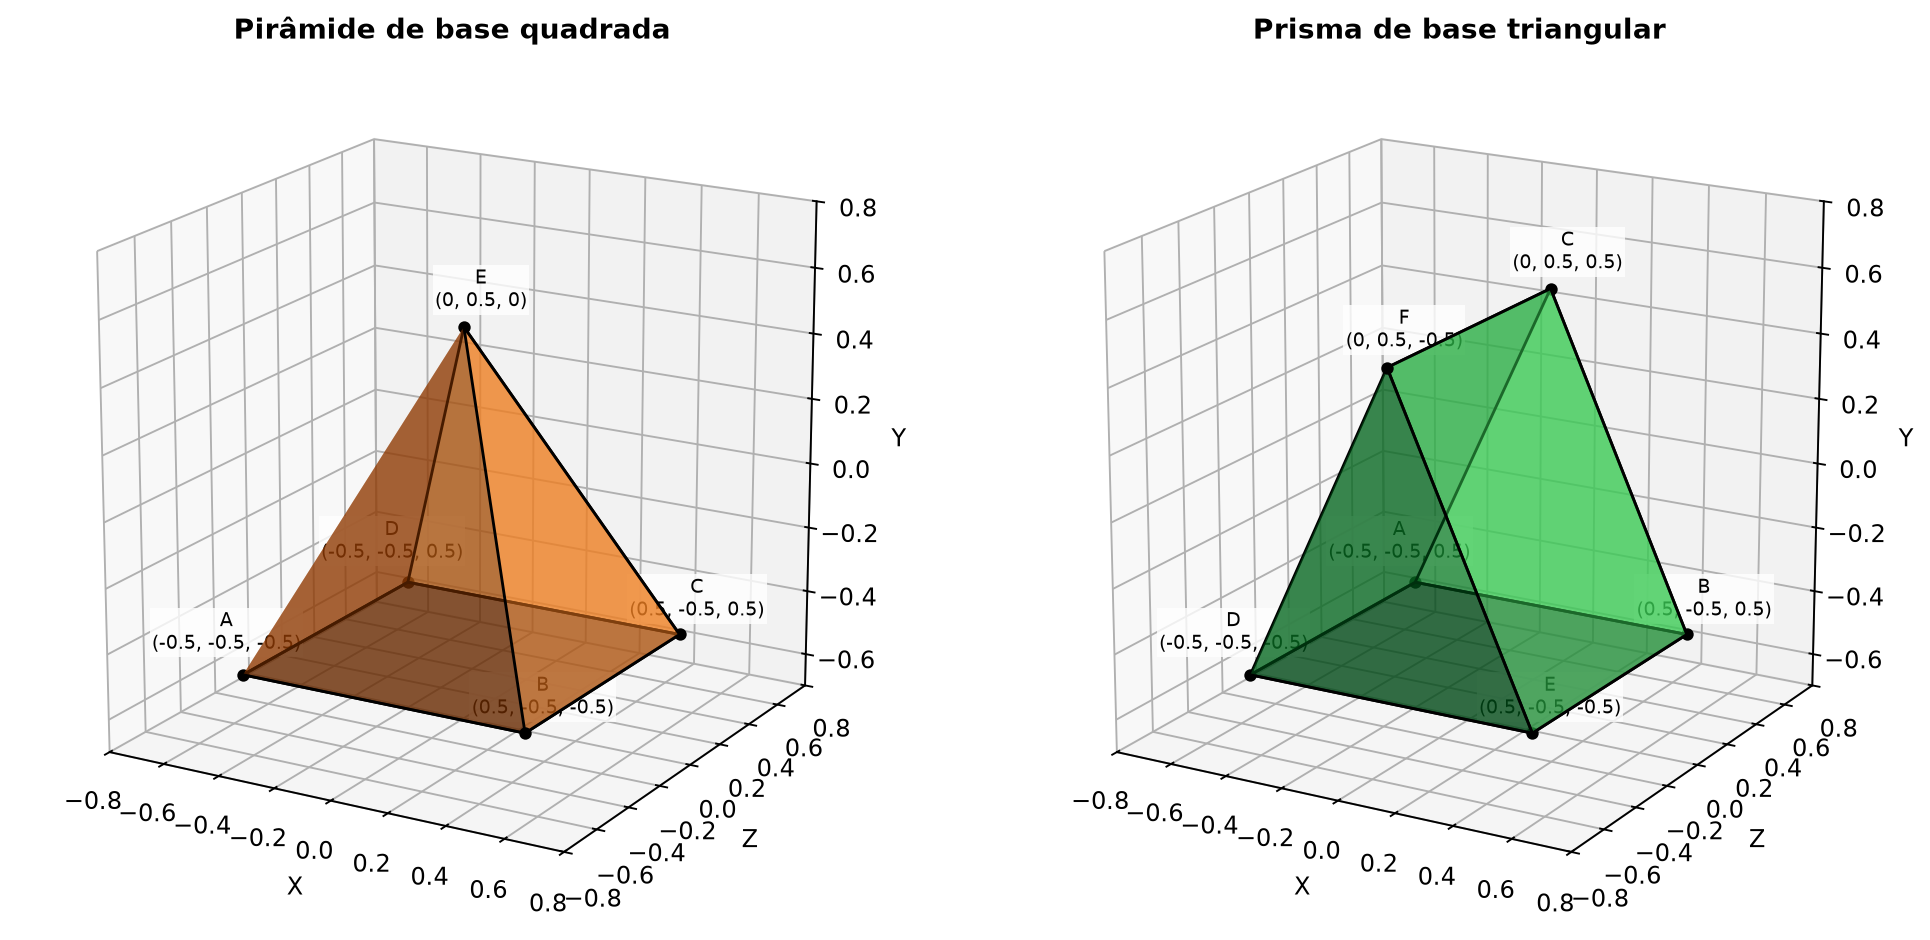
\includegraphics[width=\textwidth]{images/geometria_solidos.png}
    \caption{Vértices da pirâmide e do prisma no sistema do objeto. As cores são as mesmas usadas nos programas. O eixo $Y$ do OpenGL foi desenhado na vertical.}
    \label{fig:geometria}
\end{figure}

Como a GPU só desenha triângulos, cada face precisa ser dividida: um triângulo é desenhado direto, e um quadrilátero é dividido em dois triângulos pela diagonal. A Tabela~\ref{tab:contagem} resume a quantidade de vértices e triângulos de cada sólido.

\begin{table}[H]
\centering
\caption{Quantidade de faces, vértices e triângulos de cada sólido.}
\label{tab:contagem}
\begin{tabular}{lcccc}
\toprule
\textbf{Sólido} & \textbf{Faces} & \textbf{Cantos distintos} & \textbf{Vértices no VBO} & \textbf{Triângulos} \\
\midrule
Cubo (aula) & 6 & 8 & 24 & 12 \\
Pirâmide    & 5 & 5 & 16 & 6  \\
Prisma      & 5 & 6 & 18 & 8  \\
\bottomrule
\end{tabular}
\end{table}

A coluna ``Vértices no VBO'' é maior que a de cantos distintos porque cada vértice carrega também uma cor. Um mesmo canto pertence a várias faces de cores diferentes, então ele precisa ser repetido uma vez para cada face. É isso que dá a cada face uma cor sólida e faz as arestas do sólido ficarem visíveis.

\section{Metodologia}

O código está nos arquivos \texttt{piramide\_3d.py} e \texttt{prisma\_3d.py}. Os dois são iguais em quase tudo: as únicas diferenças são os vértices, os índices, o título da janela e alguns comentários. Por isso, nesta seção o código da pirâmide é apresentado por inteiro, na ordem em que aparece no arquivo, e do prisma são mostradas apenas as partes que mudam. A numeração das linhas nas listagens é a mesma dos arquivos originais.

\subsection{Materiais e Configuração}

O código foi desenvolvido em \textit{Python} com três bibliotecas: \texttt{glfw}, para criar a janela e ler o teclado; \texttt{PyOpenGL}, para enviar os dados e os comandos de desenho para a placa de vídeo; e \texttt{NumPy}, para montar as matrizes e os vetores de vértices. A instalação é feita com:

\begin{lstlisting}[style=pythonstyle, numbers=none]
pip install glfw PyOpenGL numpy
\end{lstlisting}

As importações estão na Listagem~\ref{lst:imports}. O módulo \texttt{OpenGL.GL} é importado com \texttt{*}, como no exemplo da aula, para que as funções e constantes do OpenGL (\texttt{glClear}, \texttt{GL\_TRIANGLES}, etc.) possam ser usadas com o mesmo nome da documentação oficial.

\lstinputlisting[style=pythonstyle, firstline=1, lastline=4, firstnumber=1, caption={Importação das bibliotecas}, label={lst:imports}]{code/piramide_3d.py}

\subsection{Shaders}

Os \textit{shaders} são pequenos programas escritos em GLSL que rodam dentro da placa de vídeo. Eles ficam guardados como texto em duas variáveis do Python (Listagem~\ref{lst:shaders}) e são compilados depois que a janela é criada.

O \textit{vertex shader} roda uma vez para cada vértice. Ele recebe a posição (\texttt{aPos}) e a cor (\texttt{aColor}) do vértice e a matriz \texttt{MVP}, que é a mesma para todos os vértices e por isso é declarada como \texttt{uniform}. A linha \texttt{gl\_Position = MVP * vec4(aPos, 1.0)} é exatamente a Equação~\ref{eq:mvp}: o \texttt{1.0} é a coordenada homogênea $w = 1$ acrescentada ao ponto. A cor é apenas repassada adiante.

O \textit{fragment shader} roda uma vez para cada pixel coberto por um triângulo e simplesmente pinta o pixel com a cor recebida, com opacidade total (\texttt{1.0}).

\lstinputlisting[style=pythonstyle, firstline=6, lastline=29, firstnumber=6, caption={Código dos shaders de vértice e de fragmento}, label={lst:shaders}]{code/piramide_3d.py}

\subsection{Funções das Matrizes}

As matrizes das Equações~\ref{eq:matrizes} e~\ref{eq:perspectiva} foram implementadas como funções (Listagem~\ref{lst:matrizes}), todas com o tipo \texttt{np.float32}, que é o tipo de número usado pela placa de vídeo:

\begin{itemize}
    \item \texttt{matriz\_perspectiva(fov, aspecto, perto, longe)}: começa com uma matriz de zeros e preenche apenas as cinco posições que não são nulas na Equação~\ref{eq:perspectiva}, incluindo o $-1$ em \texttt{m[3, 2]} que copia $-z$ para $w$;
    \item \texttt{matriz\_translacao(x, y, z)}: coloca o deslocamento na quarta coluna da identidade $4\times4$;
    \item \texttt{matriz\_rotacao\_x(graus)} e \texttt{matriz\_rotacao\_y(graus)}: convertem o ângulo para radianos com \texttt{np.radians}, calculam o seno e o cosseno uma única vez e montam as matrizes $R_x$ e $R_y$.
\end{itemize}

\lstinputlisting[style=pythonstyle, firstline=31, lastline=69, firstnumber=31, caption={Funções que geram as matrizes de perspectiva, translação e rotação}, label={lst:matrizes}]{code/piramide_3d.py}

\subsection{Janela e Contexto OpenGL}

A função \texttt{main} começa usando o GLFW (Listagem~\ref{lst:janela}). Primeiro, \texttt{glfw.init()} inicializa a biblioteca. Em seguida, os três \texttt{window\_hint} pedem um contexto OpenGL 3.3 no perfil \textit{Core}, que é a versão exigida pela linha \texttt{\#version 330 core} dos shaders. A janela de $800\times600$ pixels é criada e, se isso falhar, o programa encerra o GLFW e termina.

Depois disso, \texttt{glfw.make\_context\_current} diz ao OpenGL que os próximos comandos de desenho são para essa janela. O \texttt{glfw.swap\_interval(1)} ativa o VSync, que limita o programa à taxa de atualização do monitor (normalmente 60 quadros por segundo). Isso é importante porque o giro é feito em graus por quadro: sem o VSync, o sólido giraria rápido demais em computadores mais rápidos. Por último, \texttt{glEnable(GL\_DEPTH\_TEST)} liga o Z-Buffer, que guarda a profundidade de cada pixel e garante que uma face da frente sempre cubra uma face de trás, independentemente da ordem em que os triângulos são desenhados.

\lstinputlisting[style=pythonstyle, firstline=71, lastline=87, firstnumber=71, caption={Inicialização do GLFW, criação da janela e do contexto OpenGL}, label={lst:janela}]{code/piramide_3d.py}

\subsection{Compilação dos Shaders}

Na Listagem~\ref{lst:compilar}, os dois shaders são compilados e ligados em um único programa da GPU, guardado na variável \texttt{shader}. Em relação ao código da aula, foi acrescentado o parâmetro \texttt{validate=False}. Sem ele, o PyOpenGL valida o programa logo após a compilação, antes de existir um VAO ligado. Como o perfil \textit{Core} exige um VAO, essa validação falha em alguns drivers com o erro \textit{``No vertex array object bound''}, mesmo que o programa esteja correto. O desenho em si não é afetado, pois o VAO é criado e ligado antes de qualquer chamada de desenho.

\lstinputlisting[style=pythonstyle, firstline=89, lastline=93, firstnumber=89, caption={Compilação e ligação dos shaders}, label={lst:compilar}]{code/piramide_3d.py}

\subsection{Vértices da Pirâmide}

A Listagem~\ref{lst:vertices_piramide} define os vértices da pirâmide em um único vetor do NumPy. Cada linha é um vértice com seis números: as coordenadas $X$, $Y$, $Z$ e a cor $R$, $G$, $B$ (com valores entre 0 e 1). São 16 vértices: 4 para a base e 3 para cada uma das quatro faces laterais.

As cores seguem a mesma ideia do cubo da aula, que usava tons de azul, mas aqui em tons de laranja: a base, que fica quase sempre virada para baixo, recebe um laranja quase preto, como se estivesse na sombra, e cada face lateral recebe um tom diferente. Como o programa não calcula iluminação, essa diferença de tons é o que permite enxergar onde termina uma face e começa a outra.

\lstinputlisting[style=pythonstyle, firstline=95, lastline=125, firstnumber=95, caption={Vértices da pirâmide (posição e cor)}, label={lst:vertices_piramide}]{code/piramide_3d.py}

\subsection{Índices da Pirâmide}

Os índices (Listagem~\ref{lst:indices_piramide}) dizem quais vértices formam cada triângulo. Cada grupo de três números é um triângulo. A base é um quadrado, então ela é dividida em dois triângulos pela diagonal: (0, 1, 2) e (2, 3, 0). As faces laterais já são triângulos e usam os vértices na ordem em que foram declarados. No total são 6 triângulos e 18 índices. O tipo \texttt{np.uint32} foi usado porque é o tipo informado depois na chamada de desenho (\texttt{GL\_UNSIGNED\_INT}).

\lstinputlisting[style=pythonstyle, firstline=127, lastline=134, firstnumber=127, caption={Índices que ligam os vértices da pirâmide em triângulos}, label={lst:indices_piramide}]{code/piramide_3d.py}

\subsection{Envio dos Dados para a Placa de Vídeo}

Na Listagem~\ref{lst:buffers}, os vértices e os índices são copiados para a memória da placa de vídeo. São criados três objetos:

\begin{itemize}
    \item \textbf{VBO} (\textit{Vertex Buffer Object}): guarda o vetor de vértices;
    \item \textbf{EBO} (\textit{Element Buffer Object}): guarda o vetor de índices;
    \item \textbf{VAO} (\textit{Vertex Array Object}): guarda a configuração de como os dados do VBO devem ser lidos. Enquanto o VAO está ligado, as configurações feitas ficam salvas nele.
\end{itemize}

As duas chamadas a \texttt{glVertexAttribPointer} explicam ao OpenGL o formato de cada vértice. O \texttt{passo} é o tamanho de um vértice inteiro em bytes ($6 \times 4 = 24$ bytes, pois cada \texttt{float32} ocupa 4 bytes). O atributo 0 (\texttt{aPos} no shader) são os 3 primeiros números de cada vértice, começando no byte 0, e o atributo 1 (\texttt{aColor}) são os 3 números seguintes, começando no byte $3 \times 4 = 12$. Ao final, o VAO é desligado com \texttt{glBindVertexArray(0)}, para que nenhuma configuração posterior o altere sem querer.

\lstinputlisting[style=pythonstyle, firstline=136, lastline=155, firstnumber=136, caption={Criação dos buffers e configuração dos atributos de vértice}, label={lst:buffers}]{code/piramide_3d.py}

\subsection{Matrizes Fixas e Estado da Rotação}

Antes do laço principal (Listagem~\ref{lst:estado}), são calculadas as duas matrizes que não mudam durante a execução: a projeção, com campo de visão de $45^\circ$, proporção $800/600$ e planos de corte em 0,1 e 100; e a view, que afasta o sólido 3,5 unidades da câmera. A função \texttt{glGetUniformLocation} busca a posição da variável \texttt{MVP} dentro do programa da GPU, para que ela possa ser atualizada a cada quadro.

Os ângulos começam em $\theta_x = 25^\circ$ e $\theta_y = 45^\circ$, para que o sólido já apareça inclinado e com mais de uma face visível. A variável \texttt{velocidade} define quantos graus o sólido gira a cada quadro enquanto uma seta estiver pressionada.

\lstinputlisting[style=pythonstyle, firstline=157, lastline=167, firstnumber=157, caption={Matrizes de projeção e view e variáveis de estado da rotação}, label={lst:estado}]{code/piramide_3d.py}

\subsection{Laço Principal: Leitura do Teclado}

O laço principal (Listagem~\ref{lst:teclado}) se repete até que o usuário feche a janela, o que é verificado com \texttt{glfw.window\_should\_close}. A cada volta, \texttt{glfw.poll\_events()} busca os eventos do sistema operacional (teclas, mouse, pedido para fechar a janela).

Em seguida, \texttt{glfw.get\_key} pergunta se cada seta está pressionada \textit{naquele momento}. Isso é diferente de esperar um evento de ``tecla apertada'': enquanto a seta estiver segurada, o ângulo continua mudando a cada quadro, e o giro fica contínuo. As setas para a direita e para a esquerda giram o sólido em torno do eixo $Y$, e as setas para cima e para baixo giram em torno do eixo $X$.

\lstinputlisting[style=pythonstyle, firstline=169, lastline=181, firstnumber=169, caption={Laço principal e leitura das setas do teclado}, label={lst:teclado}]{code/piramide_3d.py}

\subsection{Laço Principal: Desenho}

A segunda metade do laço (Listagem~\ref{lst:desenho}) desenha um quadro:

\begin{enumerate}
    \item \texttt{glClearColor} e \texttt{glClear} apagam o quadro anterior, pintando o fundo de azul claro e zerando o Z-Buffer;
    \item \texttt{glUseProgram} ativa os shaders compilados;
    \item a matriz \texttt{model} é calculada com os ângulos atuais e a \texttt{MVP} é montada na ordem $P \cdot V \cdot M$ da Equação~\ref{eq:mvp};
    \item \texttt{glUniformMatrix4fv} envia a \texttt{MVP} para o shader. O NumPy guarda as matrizes linha por linha, mas o OpenGL espera coluna por coluna. Por isso a matriz é transposta com \texttt{MVP.T} antes do envio, e \texttt{np.ascontiguousarray} garante que os dados fiquem em sequência na memória;
    \item o VAO é ligado e \texttt{glDrawElements} desenha todos os triângulos de uma vez, lendo os índices do EBO;
    \item \texttt{glfw.swap\_buffers} troca o quadro que estava sendo desenhado com o que está na tela. O desenho é sempre feito em um buffer escondido e só aparece pronto, o que evita que o usuário veja o quadro pela metade.
\end{enumerate}

\lstinputlisting[style=pythonstyle, firstline=183, lastline=199, firstnumber=183, caption={Limpeza do quadro, cálculo da MVP e desenho da pirâmide}, label={lst:desenho}]{code/piramide_3d.py}

\subsection{Encerramento e Execução do Programa}

Quando a janela é fechada, o laço termina e \texttt{glfw.terminate()} libera a janela e o contexto OpenGL (Listagem~\ref{lst:main}). As duas últimas linhas fazem com que a função \texttt{main} seja executada apenas quando o arquivo é rodado diretamente (\texttt{python piramide\_3d.py}), e não quando ele é importado por outro script.

\lstinputlisting[style=pythonstyle, firstline=201, lastline=204, firstnumber=201, caption={Encerramento do GLFW e ponto de entrada do programa}, label={lst:main}]{code/piramide_3d.py}

\subsection{Diferenças no Prisma}

O arquivo \texttt{prisma\_3d.py} é igual ao da pirâmide, com exceção do título da janela e da geometria. Os vértices do prisma estão na Listagem~\ref{lst:vertices_prisma}. São 18 vértices: 3 para cada uma das duas bases triangulares e 4 para cada uma das três faces laterais retangulares. Desta vez foram usados tons de verde: a base da frente recebe o verde mais claro, a de trás um verde escuro e a face de baixo um verde quase preto, novamente simulando a sombra.

\lstinputlisting[style=pythonstyle, firstline=95, lastline=128, firstnumber=95, caption={Vértices do prisma (posição e cor)}, label={lst:vertices_prisma}]{code/prisma_3d.py}

Nos índices (Listagem~\ref{lst:indices_prisma}), as duas bases são triângulos e usam um grupo de três índices cada. As três faces laterais são retângulos e, assim como a base da pirâmide, cada uma é dividida em dois triângulos pela diagonal, por exemplo (6, 7, 8) e (8, 9, 6). No total são 8 triângulos e 24 índices. Como \texttt{glDrawElements} recebe \texttt{len(indices)}, a chamada de desenho não precisou ser alterada: ela se ajusta sozinha à quantidade de índices de cada sólido.

\lstinputlisting[style=pythonstyle, firstline=130, lastline=137, firstnumber=130, caption={Índices que ligam os vértices do prisma em triângulos}, label={lst:indices_prisma}]{code/prisma_3d.py}

\section{Resultados}

Os dois programas foram executados e abriram uma janela de $800\times600$ pixels com o sólido no centro, que pode ser girado com as setas do teclado. Para registrar o resultado, as imagens foram capturadas diretamente do framebuffer do OpenGL (com \texttt{glReadPixels}) em quatro momentos: na pose inicial e depois de segurar as setas por alguns quadros. Como cada quadro gira $2^\circ$, segurar uma seta por 45 quadros gira o sólido $90^\circ$. As imagens foram recortadas ao redor do sólido.

A Figura~\ref{fig:piramide} mostra a pirâmide. Na pose inicial (a), aparecem duas faces laterais e o ápice. Depois de girar $90^\circ$ em torno de $Y$ (b), o contorno é o mesmo, já que a pirâmide é simétrica, mas as cores mudaram: a face esquerda, que em (a) estava do lado esquerdo da imagem, passou para o lado direito, a face frontal saiu de vista e a face traseira entrou no lugar dela. Em (c), a pirâmide foi tombada com a seta para cima e a base escura aparece sozinha, cobrindo as faces laterais que ficaram atrás dela; isso confirma que o Z-Buffer está funcionando. Em (d), a pirâmide foi tombada para o outro lado com a seta para baixo e agora o ápice aponta para a câmera: as faces frontal e direita aparecem abertas a partir dele, e as outras duas surgem apenas como faixas finas na borda inferior.

\begin{figure}[H]
    \centering
    \begin{subfigure}[b]{0.24\textwidth}
        
\includegraphics[width=\textwidth]{images/piramide_inicial.png}
        \caption{$\theta_x = 25^\circ$, $\theta_y = 45^\circ$}
    \end{subfigure}
    \hfill
    \begin{subfigure}[b]{0.24\textwidth}
        
\includegraphics[width=\textwidth]{images/piramide_direita.png}
        \caption{$\theta_x = 25^\circ$, $\theta_y = 135^\circ$}
    \end{subfigure}
    \hfill
    \begin{subfigure}[b]{0.24\textwidth}
        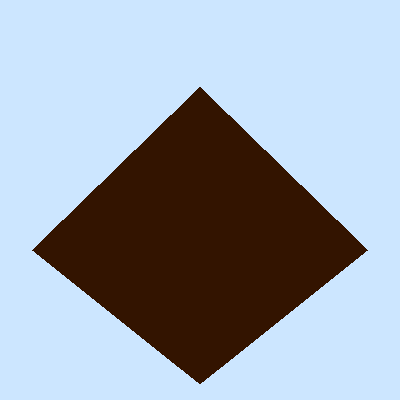
\includegraphics[width=\textwidth]{images/piramide_cima.png}
        \caption{$\theta_x = -65^\circ$, $\theta_y = 135^\circ$}
    \end{subfigure}
    \hfill
    \begin{subfigure}[b]{0.24\textwidth}
        
\includegraphics[width=\textwidth]{images/piramide_baixo.png}
        \caption{$\theta_x = 115^\circ$, $\theta_y = 135^\circ$}
    \end{subfigure}
    \caption{Pirâmide: (a) pose inicial; (b) após 45 quadros com a seta para a direita; (c) após mais 45 quadros com a seta para cima; (d) após mais 90 quadros com a seta para baixo.}
    \label{fig:piramide}
\end{figure}

A Figura~\ref{fig:prisma} mostra o prisma com a mesma sequência de teclas. Na pose inicial (a) aparecem a base triangular da frente, em verde claro, e a face inclinada esquerda, que ocupa a maior parte da imagem. Em (b), depois do giro em $Y$, a face inclinada esquerda continua visível, mas agora ao lado da base de trás, em verde escuro. Em (c), o prisma é visto por baixo e a face inferior, a mais escura, ocupa quase toda a imagem, com apenas uma faixa da base de trás aparecendo na borda. Em (d), o prisma tombou para o outro lado e passam a aparecer a face inclinada direita, a base da frente e uma faixa fina da face inclinada esquerda.

\begin{figure}[H]
    \centering
    \begin{subfigure}[b]{0.24\textwidth}
        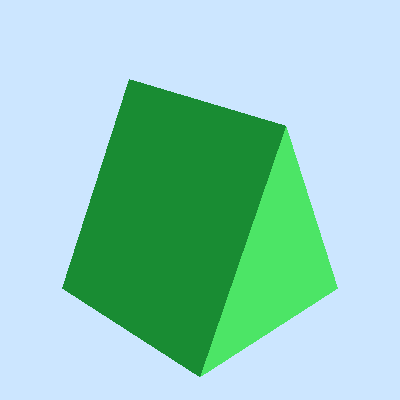
\includegraphics[width=\textwidth]{images/prisma_inicial.png}
        \caption{$\theta_x = 25^\circ$, $\theta_y = 45^\circ$}
    \end{subfigure}
    \hfill
    \begin{subfigure}[b]{0.24\textwidth}
        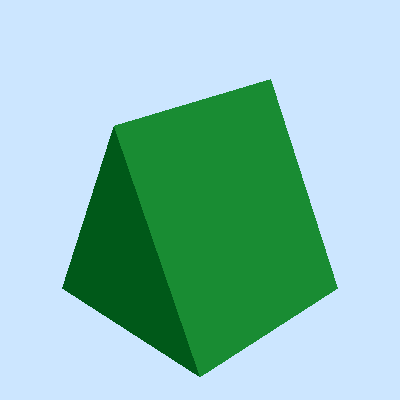
\includegraphics[width=\textwidth]{images/prisma_direita.png}
        \caption{$\theta_x = 25^\circ$, $\theta_y = 135^\circ$}
    \end{subfigure}
    \hfill
    \begin{subfigure}[b]{0.24\textwidth}
        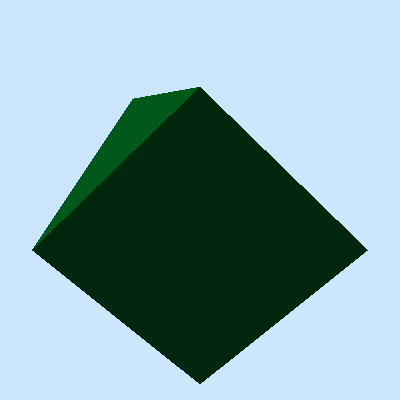
\includegraphics[width=\textwidth]{images/prisma_cima.png}
        \caption{$\theta_x = -65^\circ$, $\theta_y = 135^\circ$}
    \end{subfigure}
    \hfill
    \begin{subfigure}[b]{0.24\textwidth}
        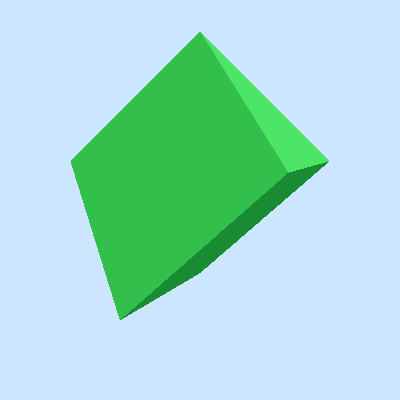
\includegraphics[width=\textwidth]{images/prisma_baixo.png}
        \caption{$\theta_x = 115^\circ$, $\theta_y = 135^\circ$}
    \end{subfigure}
    \caption{Prisma: (a) pose inicial; (b) após 45 quadros com a seta para a direita; (c) após mais 45 quadros com a seta para cima; (d) após mais 90 quadros com a seta para baixo.}
    \label{fig:prisma}
\end{figure}

Para conferir as contas, a matriz MVP da pose inicial foi calculada com as mesmas funções do programa:

\begin{equation}
MVP = \begin{bmatrix}
1{,}2803 & 0      & 1{,}2803  & 0 \\
0{,}7215 & 2{,}188 & -0{,}7215 & 0 \\
0{,}6421 & -0{,}4235 & -0{,}6421 & 3{,}3068 \\
0{,}6409 & -0{,}4226 & -0{,}6409 & 3{,}5
\end{bmatrix}
\end{equation}

Aplicando essa matriz ao ápice da pirâmide, $[0;\ 0{,}5;\ 0;\ 1]^T$, obtém-se $[0;\ 1{,}094;\ 3{,}095;\ 3{,}289]^T$. A coordenada $w$ deixou de ser 1 e passou a valer 3,289, que é a distância do ápice até a câmera. Dividindo por $w$ (Equação~\ref{eq:divisao}), o ápice vai para $x = 0$ e $y = 0{,}333$ na tela normalizada, que vai de $-1$ a $1$. Convertendo para a janela de $800\times600$, isso corresponde ao pixel $(400,\ 200)$, que é exatamente onde o ápice aparece na Figura~\ref{fig:piramide}(a) (o recorte começa no pixel $(200,\ 100)$ da janela). Da mesma forma, os cantos $A = (-0{,}5;\ -0{,}5;\ -0{,}5)$ e $C = (0{,}5;\ -0{,}5;\ 0{,}5)$ caem nos pixels $(262,\ 388)$ e $(538,\ 388)$, simétricos em relação ao centro da janela, como esperado para $\theta_y = 45^\circ$.

\section{Conclusão}

A atividade mostrou que, depois que a estrutura do programa com GLFW e OpenGL está pronta, desenhar um novo sólido é basicamente um problema de geometria: definir os vértices, escolher as cores das faces e dividir cada face em triângulos. A janela, o contexto, os shaders, os buffers, as matrizes e o laço principal do cubo da aula foram reaproveitados sem mudanças, e mesmo a chamada de desenho se adaptou sozinha à quantidade de índices de cada sólido.

Também ficou claro como as coordenadas homogêneas da Aula 14 são usadas na prática. Elas permitem juntar rotação, translação e perspectiva em uma única matriz $4\times4$, que a placa de vídeo aplica a todos os vértices com uma só multiplicação. A coordenada $w$, que nas transformações 2D era sempre 1, passa a guardar a distância até a câmera, e a divisão por $w$ é o que faz os objetos distantes parecerem menores. Por fim, o GLFW cumpriu as três funções vistas em aula: abriu a janela, criou o contexto OpenGL e entregou ao programa as setas do teclado que controlam a rotação.

\begin{thebibliography}{9}

\bibitem{rodrigo_glfw}
RODRIGO, Raulivan. \textbf{GLFW - Graphics Library Framework}. Notas de Aula (15 - GLFW - Graphics Library Framework.pdf). Departamento de Computação, Centro Federal de Educação Tecnológica de Minas Gerais (CEFET-MG), 2026.

\bibitem{rodrigo_homog}
RODRIGO, Raulivan. \textbf{Coordenadas Homogêneas}. Notas de Aula (14 - Coordenadas Homogêneas.pdf). Departamento de Computação, Centro Federal de Educação Tecnológica de Minas Gerais (CEFET-MG), 2026.

\bibitem{rodrigo_cubo}
RODRIGO, Raulivan. \textbf{cubo\_3d.py}. Repositório computacao-grafica-python. Disponível em: \url{https://github.com/raulivan/computacao-grafica-python/blob/main/AULA15/cubo_3d.py}.

\bibitem{glfw_docs}
GLFW DEVELOPMENT TEAM. \textbf{GLFW Documentation}. Disponível em: \url{https://www.glfw.org/documentation.html}.

\bibitem{pyopengl_docs}
PYOPENGL DEVELOPERS. \textbf{PyOpenGL Documentation}. Disponível em: \url{https://pyopengl.sourceforge.net/documentation/}.

\bibitem{numpy_docs}
NUMPY DEVELOPERS. \textbf{NumPy Documentation}. Disponível em: \url{https://numpy.org/doc/stable/}.

\end{thebibliography}

\end{document}
